\chapter{Initial Value Problems}

\section{The explicit midpoint rule}

Let \(f: \R\times \R^n \rightarrow \R^n\) be a smooth mapping and consider the initial value problem 
\begin{equation}\label{ivp}
y'(t) = f(t, y(t)), \quad y(a) = y_a, \quad t\in [a,b].
\end{equation}
The explicit midpoint methods is a method for computing an approximation to the solution of (\ref{ivp}), and it goes as follows: Let \(n\geq 1\) be an integer and \(h\coloneqq (b-a)/2n\). We then define recursively
\[
\xi_h(a) \coloneqq y_a, \quad \xi_h(a+h) \coloneqq \xi_h(a) + hf(a, \xi_h(a))
\]
and
\[
\xi_h(a + (i+1)h) \coloneqq \xi_h(a+(i-1)h) + 2hf(a+ih, \xi(a+ih)).
\]
Then \(\xi_h\) is an approximate solution to (\ref{ivp}) defined at \(a, a+h,\ldots ,b\). We are interested in the value \(X_f(h)\coloneqq \xi_h(b)\). It is possible to show that \(X_f(h)\) has an asymptotic expansion in \(h^2\). We have the following implementation in Python of the explicit midpoint rule for computing \(X_f(h)\).

\begin{minted}[tabsize=2, fontsize=\footnotesize]{python}
class ExplicitMidpointRule(Scheme):

	def __init__(self):
		super(ExplicitMidpointRule, self).__init__(2)

	def apply(self, ivp, n):
		h = (ivp.b - ivp.a) / (2 * n)
		y_sl = ivp.y0
		y_l = ivp.y0 + h * ivp.f(ivp.a, ivp.y0)

		for i in range(1, 2 * n):
			tmp = y_l
			y_l = y_sl + 2 * h * ivp.f(ivp.a + i * h, y_l)
			y_sl = tmp

		return y_l
\end{minted}

\section{Numerical experiments}

In this section we are going to extrapolate the explicit midpoint rule and analyze the convergence of the approximations as we extrapolate more often. Consider the initial value problem (\ref{ivp}). Let \(n_1 < n_2 < \cdots\) be some sequence of integers and \(h_i \coloneqq (b-a) / n_i\). Let \(X_{ij}\) the extrapolation table which we get from extrapolating in \(h^2\), using the points \((h_i,X_f(h_i))\). Let \(\varepsilon_i \coloneqq |X_{ii} - y(b)|\) be the absolute error. We are going to do the same convergence and efficency analysis as in the two previous chapters. We will both do the computations using high precision arithmetic with \(500\) correct digits and also in standard double precision.\\

%If \((a_n)\) is the sequence we use then the number of \(f\)-evaluations is %\(N_n = \sum_{k=1}^n 2\cdot a_n\). Thus for the harmonic sequence we have %\(N_n = n(n+1) \approx n^2\) for \(n\) large so if \(\varepsilon_n \sim %A\exp (-cN_n^q)\) then \(\varepsilon_n \sim A\exp(-cn^{2q})\) for large %\(n\). For the Romberg sequence then \(N_n = 2^{n+1} - 1\) so if %\(\varepsilon_n\sim A\exp(-cN_n^q)\) then \(\varepsilon_n \sim %A\exp(-c2^{nq})\) for large \(n\).\\

In those cases where we do not have an analytic solution to the equations, we computed a reference solution up to \(500\) significant digits. We did that by using extrapolation with the harmonic sequence and estimating the error as the difference between successive terms in the sequence of approximations.\\

Now we will consider the results of the experiments.

\subsection{Exponential growth}
First we will consider the following initial value problem:
\begin{equation}\label{42}
y'(x) = y(x),\quad y(0) = 0, \quad x\in [0,1]
\end{equation}
whose solution is the analytic function \(y(x) = e^x\).

\begin{figure}[H]
\centering
\begin{minipage}{0.45\textwidth}
\centering
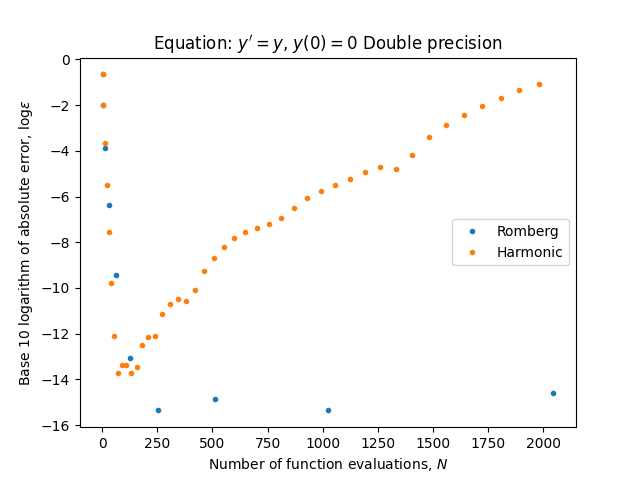
\includegraphics[scale=0.45]{emr_plots/exp_growth.png}
\end{minipage}
\begin{minipage}{0.45\textwidth}
\centering
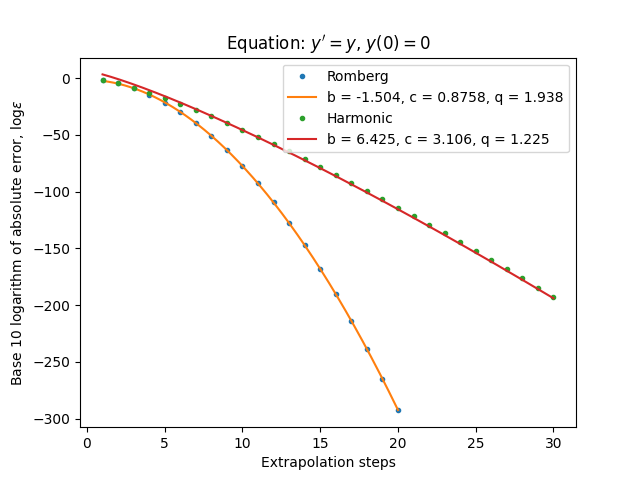
\includegraphics[scale=0.45]{emr_plots/exp_growth_hp_steps.png}
\end{minipage}
\end{figure}

\begin{figure}[H]
\centering
\begin{minipage}{0.45\textwidth}
\centering
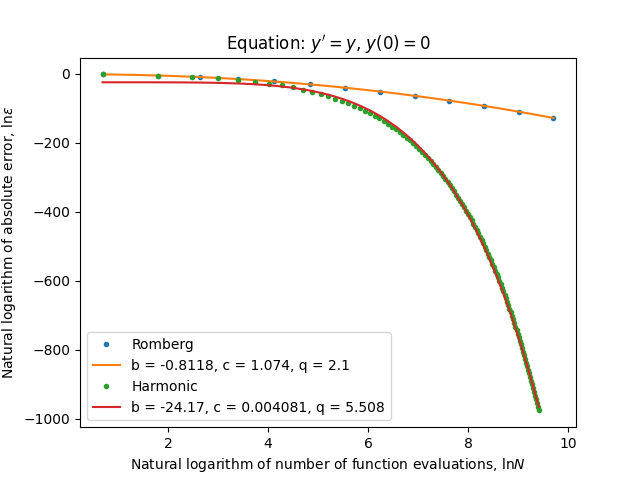
\includegraphics[scale=0.45]{emr_plots/exp_growth_hp_log_log_pow_fit_trend.png}
\end{minipage}
\begin{minipage}{0.45\textwidth}
\centering
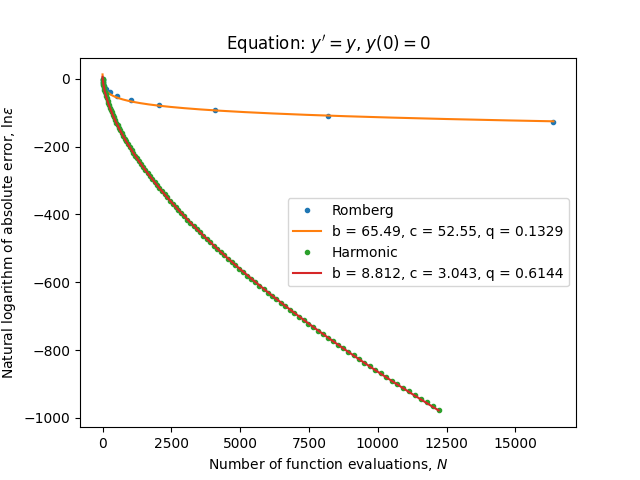
\includegraphics[scale=0.45]{emr_plots/exp_growth_hp_trend.png}
\end{minipage}
\end{figure}

\begin{table}[H]
    \centering
    \begin{tabular}{c|c||c|c|c}
Sequence & Plot & \(A\)-variance & \(c\)-variance & \(q\)-variance\\\hline
Romberg & lin-ln evals-error & \(3\) & \(0.085281\) & \(0.021208\) \\
Harmonic & lin-ln evals-error & \(12.161\) & \(0.021332\) & \(0.001013\) \\
Romberg & lin-ln steps-error & \(0.077032\) & \(0.0008956\) & \(3.583e-05\) \\
Harmonic & lin-ln steps-error & \(11.697\) & \(0.017508\) & \(0.00078485\) \\
Romberg & ln-ln evals-error & \(0.18082\) & \(0.0019753\) & \(8.8653e-05\) \\
Harmonic & ln-ln evals-error & . & . & . \\
    \end{tabular}
    \label{tab:my_label}
\end{table}

Here we have exponential convergence in all cases. The harmonic sequence performes better than Romberg. In standard floating point arithmetic, we get down to maching level error using either sequence.

\subsection{Logistic curve}

Then we will consider the following initial value problem
\begin{equation}\label{43}
y'(x) = y(x)(1-y(x)),\quad y(0) = 1/2, \quad x\in [0,1]
\end{equation}

whose solution is the sigmoid function
\[
\sigma(x) = \frac{1}{1 + e^{-x}}
\]
which is analytic.

\begin{figure}[H]
\centering
\begin{minipage}{0.45\textwidth}
\centering
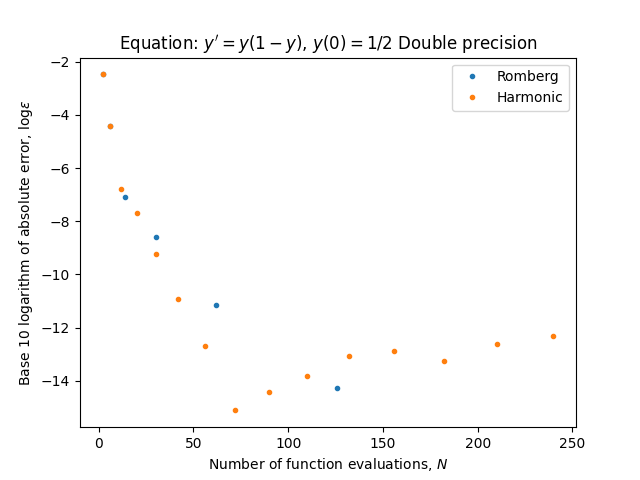
\includegraphics[scale=0.45]{emr_plots/logistic.png}
\end{minipage}
\begin{minipage}{0.45\textwidth}
\centering
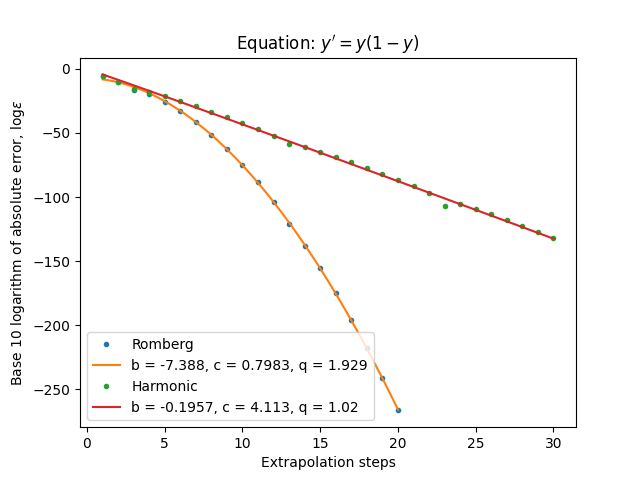
\includegraphics[scale=0.45]{emr_plots/logistic_hp_steps.png}
\end{minipage}
\end{figure}

\begin{figure}[H]
\centering
\begin{minipage}{0.45\textwidth}
\centering
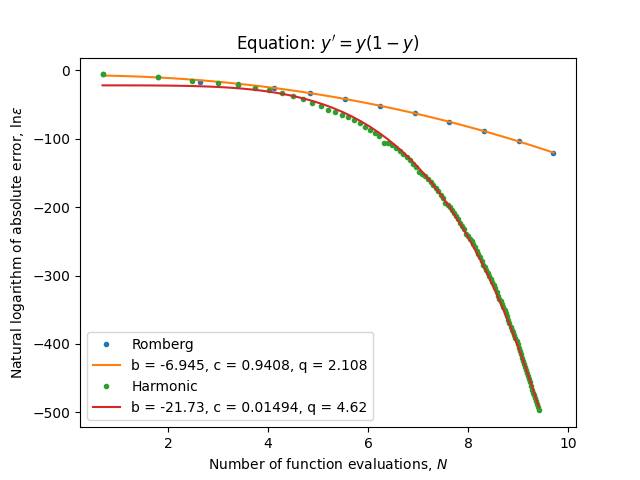
\includegraphics[scale=0.45]{emr_plots/logistic_hp_log_log_pow_fit_trend.png}
\end{minipage}
\begin{minipage}{0.45\textwidth}
\centering
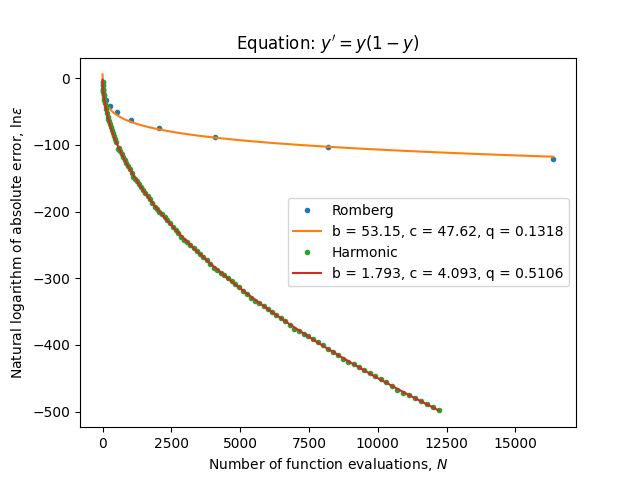
\includegraphics[scale=0.45]{emr_plots/logistic_hp_trend.png}
\end{minipage}
\end{figure}

\begin{table}[H]
    \centering
    \begin{tabular}{c|c||c|c|c}
Sequence & Plot & \(A\)-variance & \(c\)-variance & \(q\)-variance\\\hline
Romberg & lin-ln evals-error & \(2.9992\) & \(0.083333\) & \(0.020783\) \\
Harmonic & lin-ln evals-error & . & . & . \\
Romberg & lin-ln steps-error & \(0.10654\) & \(0.0019686\) & \(7.2672e-05\) \\
Harmonic & lin-ln steps-error & . & . & . \\
Romberg & ln-ln evals-error & \(0.10079\) & \(0.002435\) & \(0.00011182\) \\
Harmonic & ln-ln evals-error & . & . & . \\
    \end{tabular}
    \label{tab:my_label}
\end{table}

Here the model also fits very well, the Harmonic sequence performes better and we get down to machine level precision using either sequence in standard floating point arithmetic.

\subsection{Tangens}

Now we will consider the following equation
\begin{equation}
y'(x) = 1 + y(x)^2, \quad y(0) = 0,\quad x\in [0,1]
\end{equation}

whose solution is 
\[
y(x) \coloneqq \tan(x)
\]
which is meromorphic and we are quite far from singularites.

\begin{figure}[H]
\centering
\begin{minipage}{0.45\textwidth}
\centering
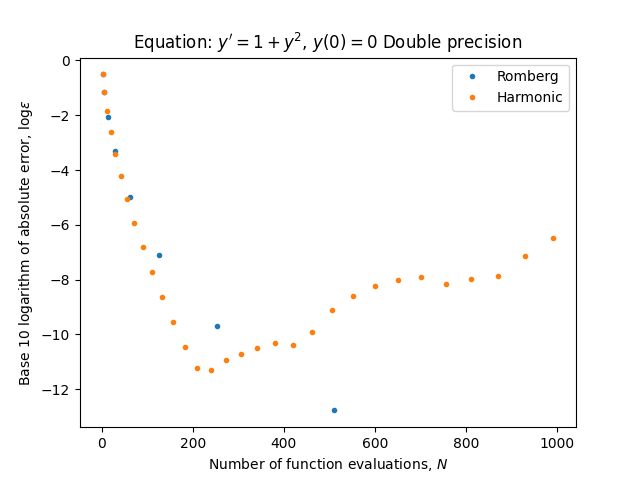
\includegraphics[scale=0.45]{emr_plots/tangens.png}
\end{minipage}
\begin{minipage}{0.45\textwidth}
\centering
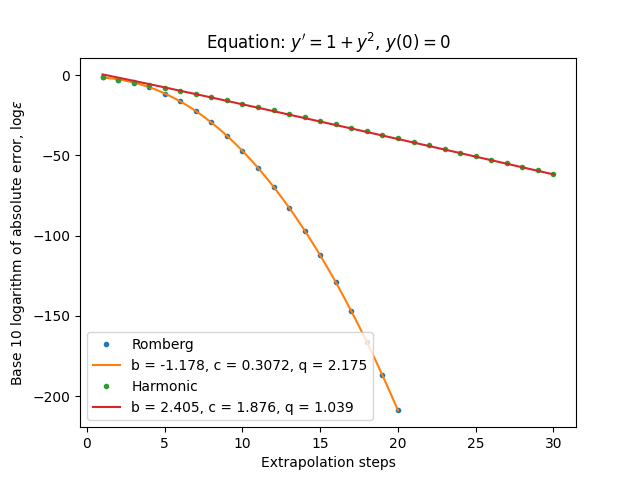
\includegraphics[scale=0.45]{emr_plots/tangens_hp_steps.png}
\end{minipage}
\end{figure}

\begin{figure}[H]
\centering
\begin{minipage}{0.45\textwidth}
\centering
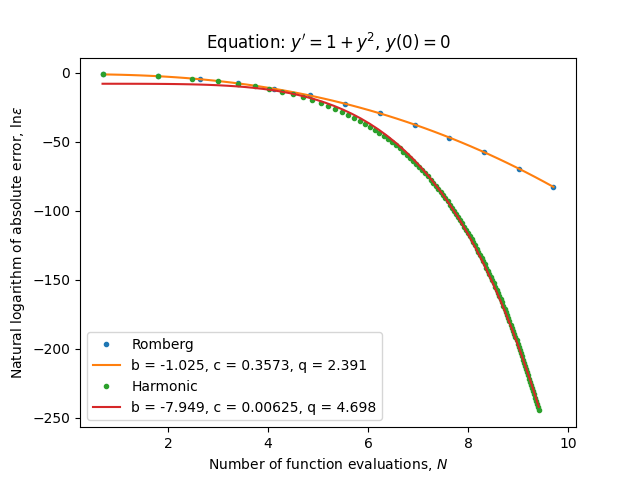
\includegraphics[scale=0.45]{emr_plots/tangens_hp_log_log_pow_fit_trend.png}
\end{minipage}
\begin{minipage}{0.45\textwidth}
\centering
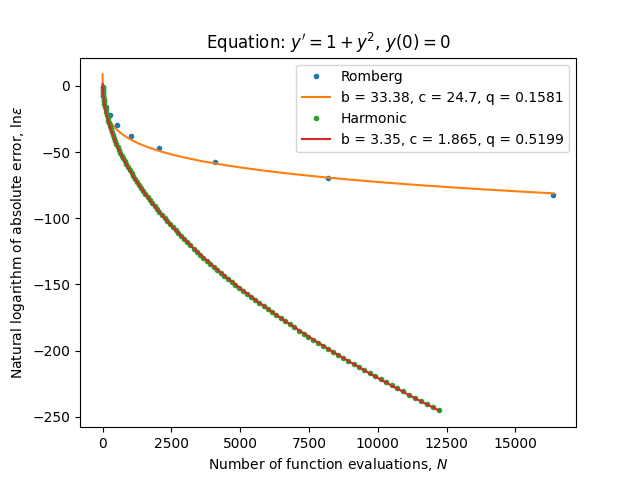
\includegraphics[scale=0.45]{emr_plots/tangens_hp_trend.png}
\end{minipage}
\end{figure}

\begin{table}[H]
    \centering
    \begin{tabular}{c|c||c|c|c}
Sequence & Plot & \(A\)-variance & \(c\)-variance & \(q\)-variance\\\hline
Romberg & lin-ln evals-error & \(2.9973\) & \(0.1255\) & \(0.024015\) \\
Harmonic & lin-ln evals-error & \(0.97512\) & \(0.014263\) & \(0.0011377\) \\
Romberg & lin-ln steps-error & \(0.0052197\) & \(0.00017853\) & \(5.4868e-06\) \\
Harmonic & lin-ln steps-error & \(0.94149\) & \(0.012584\) & \(0.00097006\) \\
Romberg & ln-ln evals-error & \(0.2211\) & \(0.0081118\) & \(0.0002882\) \\
Harmonic & ln-ln evals-error & . & . & . \\
    \end{tabular}
    \label{tab:my_label}
\end{table}

Here we also have exponential convergence in all cases. The harmonic sequence performes better than Romberg. In standard floating point arithmetic, we get down to maching level error using either sequence.

\subsection{Equation with singularity}

Now we will consider the following initial value problem:
\begin{equation}\label{46}
y'(t) = y^2(t),\quad y(0) = 1/(1+a), \quad t\in [0,1]
\end{equation}

whose solution is 
\[
y(t) = \frac{1}{1-(t-a)}.
\]
The solution is meromorphic with a pole at \(1+a\).
\begin{figure}[H]
\centering
\begin{minipage}{0.45\textwidth}
\centering
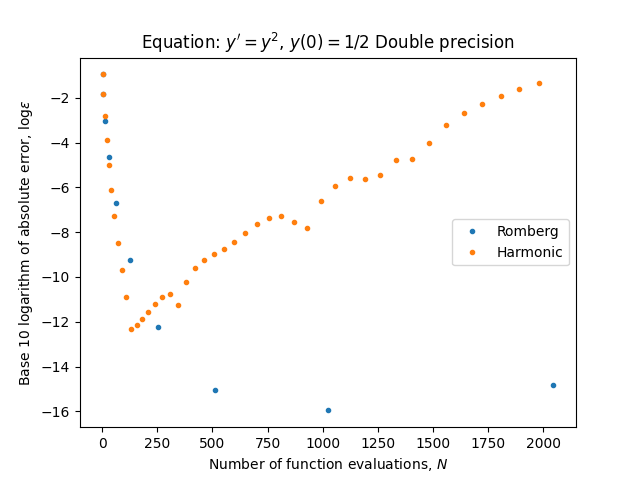
\includegraphics[scale=0.45]{emr_plots/singularity_0.png}
\end{minipage}
\begin{minipage}{0.45\textwidth}
\centering
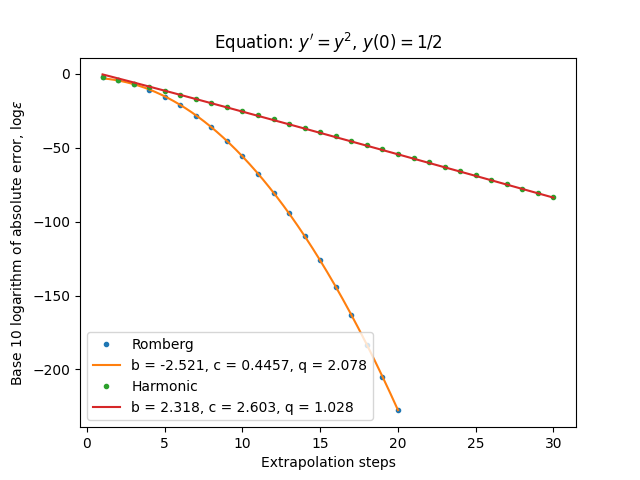
\includegraphics[scale=0.45]{emr_plots/singularity_0_hp_steps.png}
\end{minipage}
\end{figure}

\begin{figure}[H]
\centering
\begin{minipage}{0.45\textwidth}
\centering
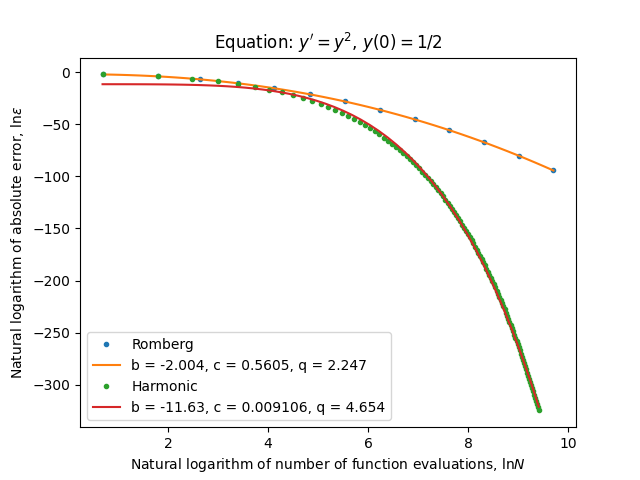
\includegraphics[scale=0.45]{emr_plots/singularity_0_hp_log_log_pow_fit_trend.png}
\end{minipage}
\begin{minipage}{0.45\textwidth}
\centering
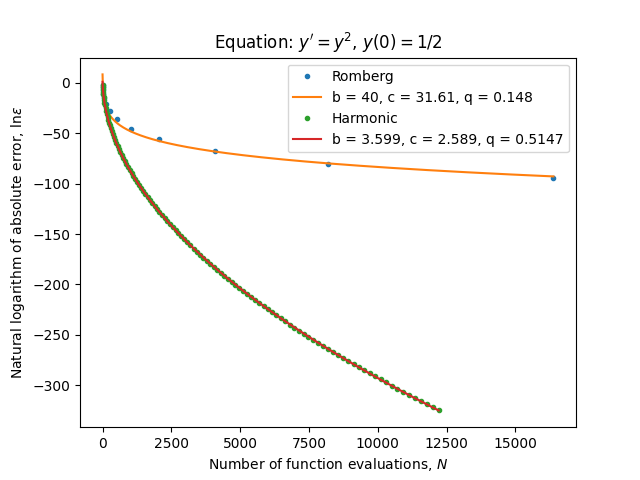
\includegraphics[scale=0.45]{emr_plots/singularity_0_hp_trend.png}
\end{minipage}
\end{figure}

\begin{table}[H]
    \centering
    \begin{tabular}{c|c||c|c|c}
Sequence & Plot & \(A\)-variance & \(c\)-variance & \(q\)-variance\\\hline
Romberg & lin-ln evals-error & \(2.999\) & \(0.097019\) & \(0.020639\) \\
Harmonic & lin-ln evals-error & \(0.91848\) & \(0.0079606\) & \(0.00061987\) \\
Romberg & lin-ln steps-error & \(0.029451\) & \(0.00085321\) & \(3.0385e-05\) \\
Harmonic & lin-ln steps-error & \(0.88236\) & \(0.0068517\) & \(0.00051693\) \\
Romberg & ln-ln evals-error & \(0.095823\) & \(0.0022727\) & \(8.8823e-05\) \\
Harmonic & ln-ln evals-error & . & . & . \\
    \end{tabular}
    \label{tab:my_label}
\end{table}

\begin{figure}[H]
\centering
\begin{minipage}{0.45\textwidth}
\centering
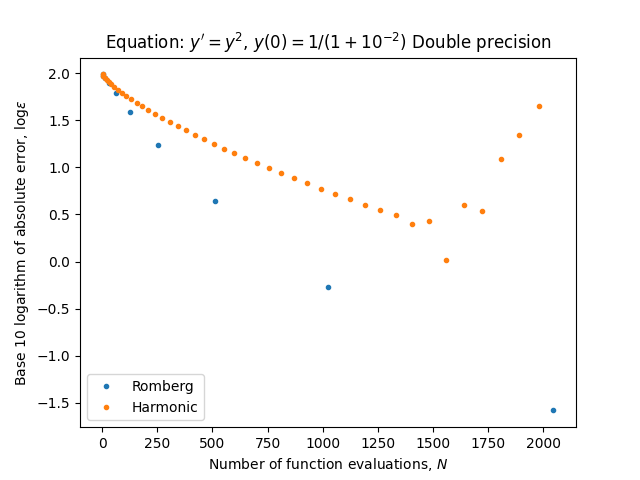
\includegraphics[scale=0.45]{emr_plots/singularity_2.png}
\end{minipage}
\begin{minipage}{0.45\textwidth}
\centering
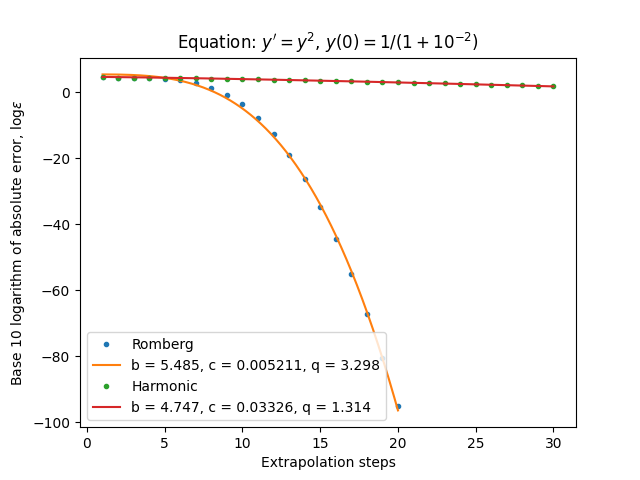
\includegraphics[scale=0.45]{emr_plots/singularity_2_hp_steps.png}
\end{minipage}
\end{figure}

\begin{figure}[H]
\centering
\begin{minipage}{0.45\textwidth}
\centering
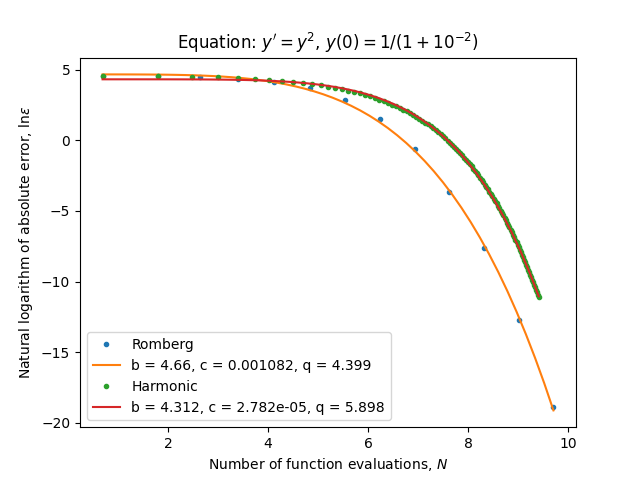
\includegraphics[scale=0.45]{emr_plots/singularity_2_hp_log_log_pow_fit_trend.png}
\end{minipage}
\begin{minipage}{0.45\textwidth}
\centering
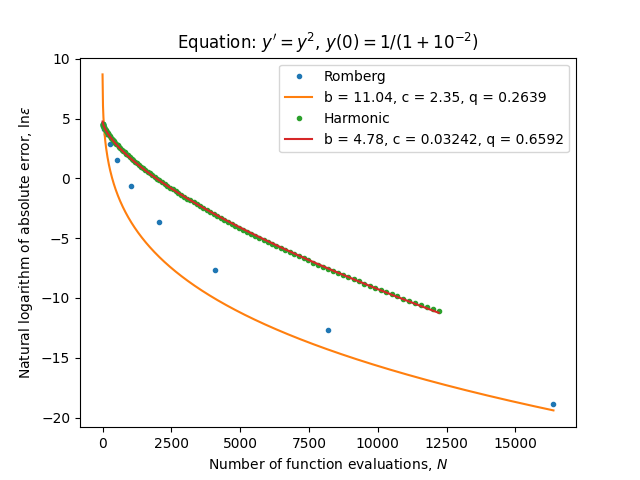
\includegraphics[scale=0.45]{emr_plots/singularity_2_hp_trend.png}
\end{minipage}
\end{figure}

\begin{table}[H]
    \centering
    \begin{tabular}{c|c||c|c|c}
Sequence & Plot & \(A\)-variance & \(c\)-variance & \(q\)-variance\\\hline
Romberg & lin-ln evals-error & \(1.1426\) & \(0.70222\) & \(0.036614\) \\
Harmonic & lin-ln evals-error & \(0.43372\) & \(0.23731\) & \(0.0075673\) \\
Romberg & lin-ln steps-error & \(0.054061\) & \(0.33189\) & \(0.0027716\) \\
Harmonic & lin-ln steps-error & \(0.43591\) & \(51.961\) & \(0.027035\) \\
Romberg & ln-ln evals-error & \(0.082011\) & \(0.43662\) & \(0.0041259\) \\
Harmonic & ln-ln evals-error & . & . & . \\
    \end{tabular}
    \label{tab:my_label}
\end{table}

\begin{figure}[H]
\centering
\begin{minipage}{0.45\textwidth}
\centering
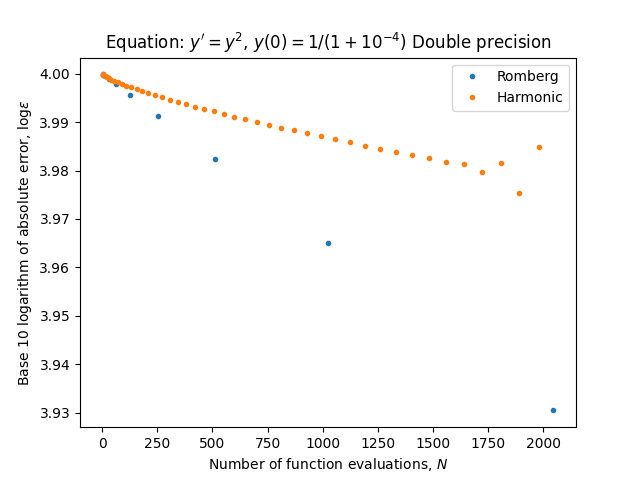
\includegraphics[scale=0.45]{emr_plots/singularity_4.png}
\end{minipage}
\begin{minipage}{0.45\textwidth}
\centering
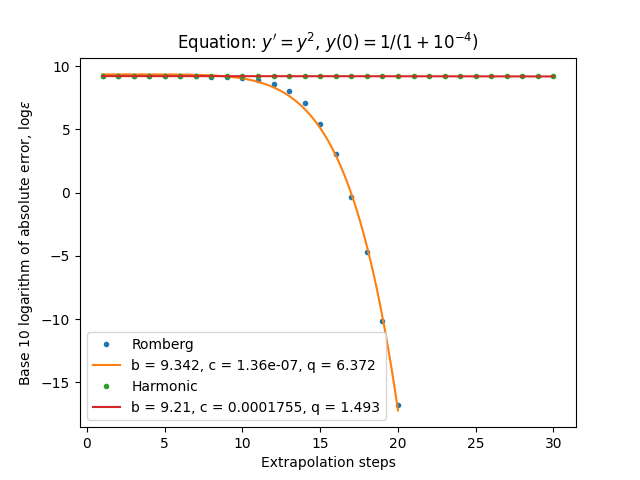
\includegraphics[scale=0.45]{emr_plots/singularity_4_hp_steps.png}
\end{minipage}
\end{figure}

\begin{figure}[H]
\centering
\begin{minipage}{0.45\textwidth}
\centering
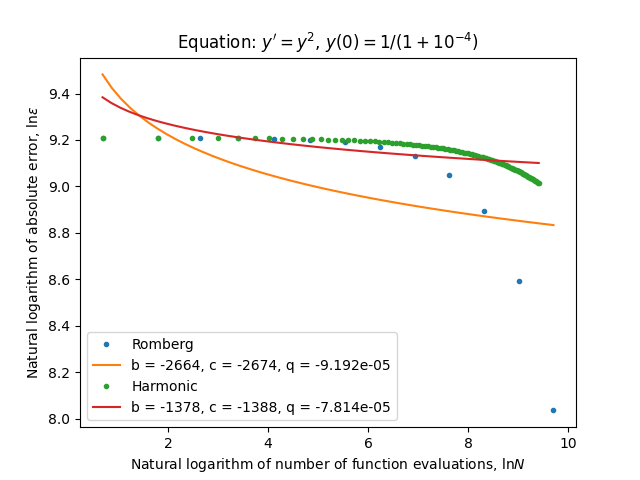
\includegraphics[scale=0.45]{emr_plots/singularity_4_hp_log_log_pow_fit_trend.png}
\end{minipage}
\begin{minipage}{0.45\textwidth}
\centering
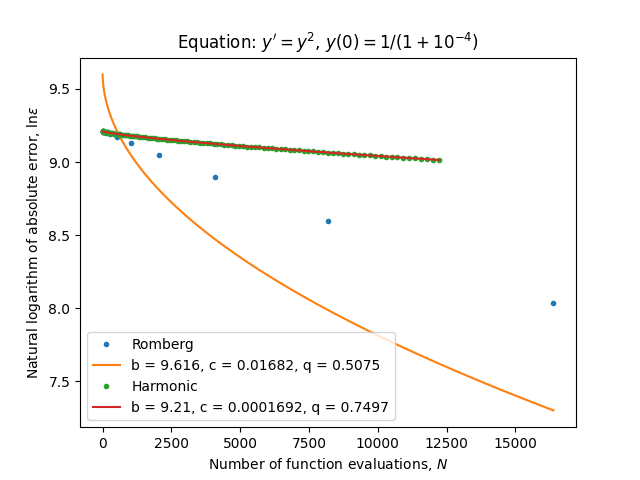
\includegraphics[scale=0.45]{emr_plots/singularity_4_hp_trend.png}
\end{minipage}
\end{figure}

\begin{table}[H]
    \centering
    \begin{tabular}{c|c||c|c|c}
Sequence & Plot & \(A\)-variance & \(c\)-variance & \(q\)-variance\\\hline
Romberg & lin-ln evals-error & \(9.0721e-07\) & \(0.011092\) & \(0.00016407\) \\
Harmonic & lin-ln evals-error & \(2.5283e-08\) & \(0.00028227\) & \(7.3639e-06\) \\
Romberg & lin-ln steps-error & \(0.33335\) & \(3\) & \(0.3392\) \\
Harmonic & lin-ln steps-error & . & . & . \\
Romberg & ln-ln evals-error & \(1\) & \(1.2321\) & \(1.0023\) \\
Harmonic & ln-ln evals-error & . & . & . \\
    \end{tabular}
    \label{tab:my_label}
\end{table}

The model fits well for large \(a\), and then the Harmonic sequence works better. But for small \(a\) we get a very poor fitting, and extremely slow convergence towards the solution. For \(a = 10^{-4}\), when considering the number of function evaluations agains the error, we can not say that we have exponential convergence because the values on the vertical axis are on much smaller scale then the ones on the horizontal axis. The fitting fails entirely when considering the number of extrapolation steps against the error with the Romberg sequence and \(a = 10^{-4}\).\\

The plot of \(q\) against \(a\) is as follows:

\begin{figure}[H]
\centering
\begin{minipage}{0.45\textwidth}
\centering
\includegraphics[scale=0.45]{emr_plots/log_p_vs_q_sing.png}
\end{minipage}
\end{figure}

\subsection{Equation with moderate singularity}

Now we will consider the following initial value problem
\begin{equation}
y'(t) = -\frac{1}{2y}, \quad y(0) = \sqrt{1+a},\quad t\in [0,1]\label{47}
\end{equation}
whose solution is 
\[
y(t) = \sqrt{1 - (t-a)}
\]
\begin{figure}[H]
\centering
\begin{minipage}{0.45\textwidth}
\centering
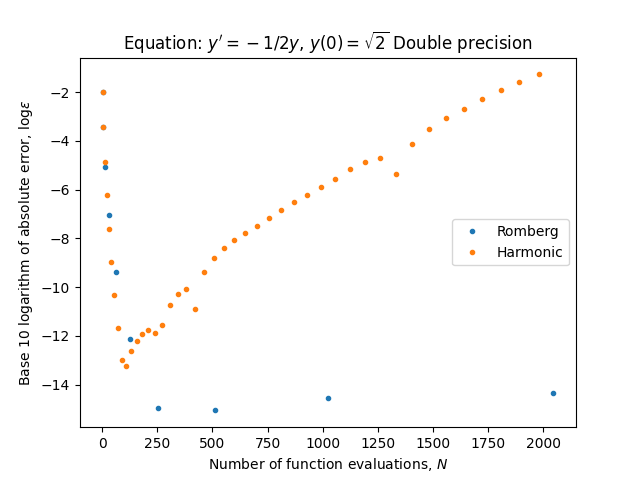
\includegraphics[scale=0.45]{emr_plots/quad_sing_0.png}
\end{minipage}
\begin{minipage}{0.45\textwidth}
\centering
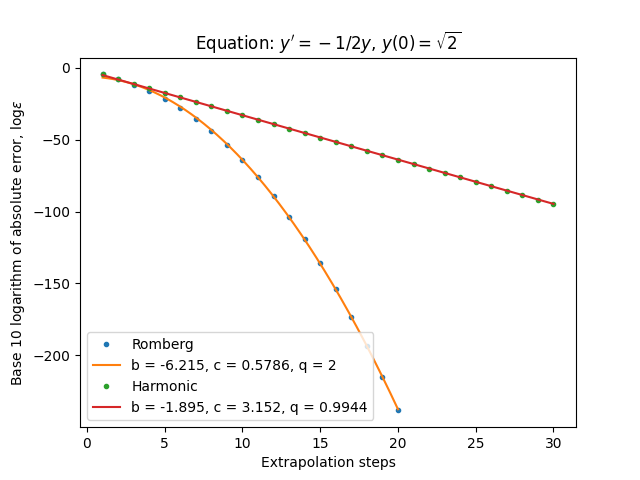
\includegraphics[scale=0.45]{emr_plots/quad_sing_0_hp_steps.png}
\end{minipage}
\end{figure}

\begin{figure}[H]
\centering
\begin{minipage}{0.45\textwidth}
\centering
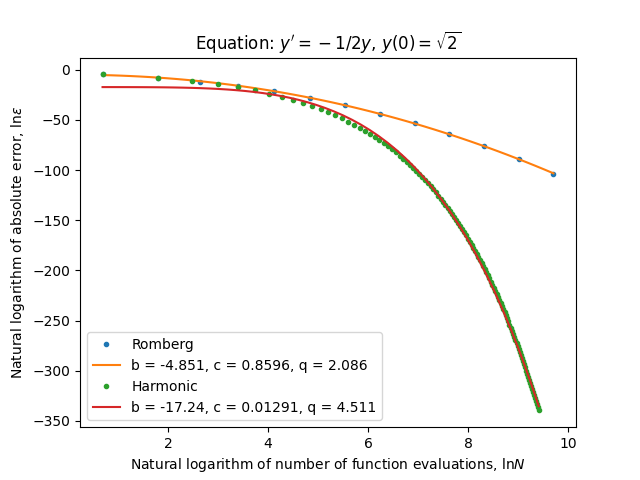
\includegraphics[scale=0.45]{emr_plots/quad_sing_0_hp_log_log_pow_fit_trend.png}
\end{minipage}
\begin{minipage}{0.45\textwidth}
\centering
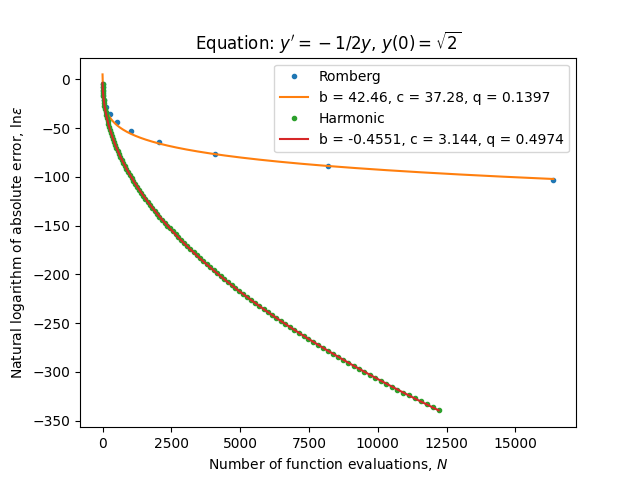
\includegraphics[scale=0.45]{emr_plots/quad_sing_0_hp_trend.png}
\end{minipage}
\end{figure}

\begin{table}[H]
    \centering
    \begin{tabular}{c|c||c|c|c}
Sequence & Plot & \(A\)-variance & \(c\)-variance & \(q\)-variance\\\hline
Romberg & lin-ln evals-error & \(2.9986\) & \(0.063649\) & \(0.014426\) \\
Harmonic & lin-ln evals-error & \(0.11952\) & \(0.00020154\) & \(1.1402e-05\) \\
Romberg & lin-ln steps-error & \(0.39967\) & \(0.0092624\) & \(0.0003485\) \\
Harmonic & lin-ln steps-error & \(0.14404\) & \(0.00026111\) & \(1.552e-05\) \\
Romberg & ln-ln evals-error & \(0.019547\) & \(0.0003673\) & \(1.5503e-05\) \\
Harmonic & ln-ln evals-error & . & . & . \\
    \end{tabular}
    \label{tab:my_label}
\end{table}

\begin{figure}[H]
\centering
\begin{minipage}{0.45\textwidth}
\centering
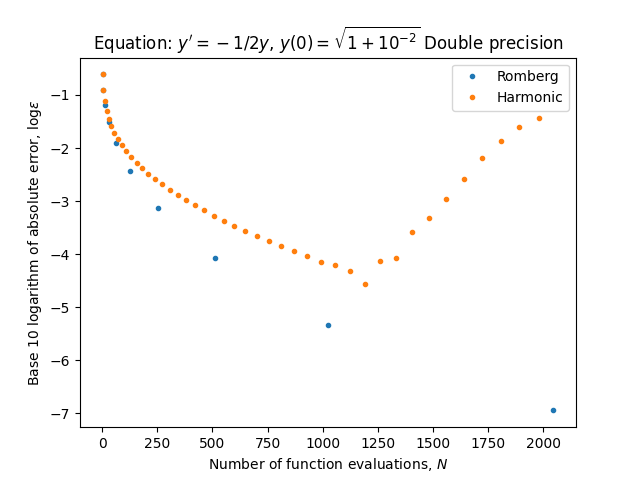
\includegraphics[scale=0.45]{emr_plots/quad_sing_2.png}
\end{minipage}
\begin{minipage}{0.45\textwidth}
\centering
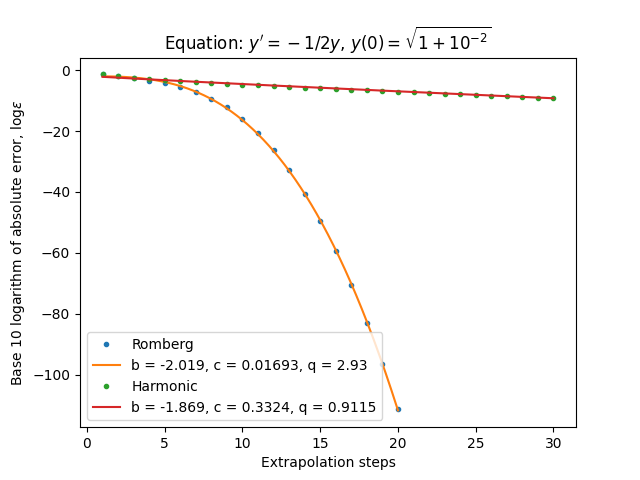
\includegraphics[scale=0.45]{emr_plots/quad_sing_2_hp_steps.png}
\end{minipage}
\end{figure}

\begin{figure}[H]
\centering
\begin{minipage}{0.45\textwidth}
\centering
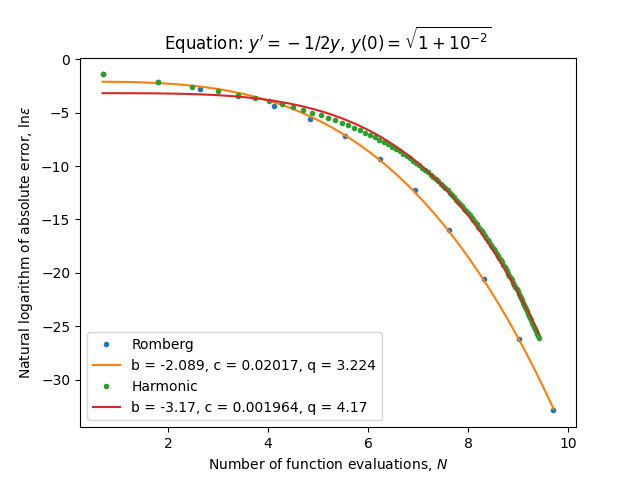
\includegraphics[scale=0.45]{emr_plots/quad_sing_2_hp_log_log_pow_fit_trend.png}
\end{minipage}
\begin{minipage}{0.45\textwidth}
\centering
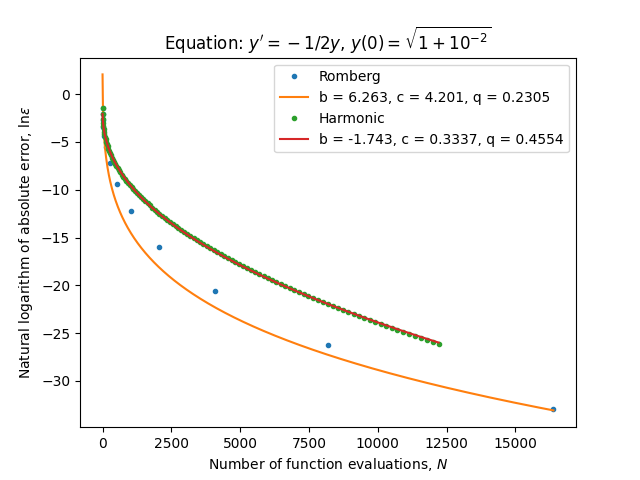
\includegraphics[scale=0.45]{emr_plots/quad_sing_2_hp_trend.png}
\end{minipage}
\end{figure}

\begin{table}[H]
    \centering
    \begin{tabular}{c|c||c|c|c}
Sequence & Plot & \(A\)-variance & \(c\)-variance & \(q\)-variance\\\hline
Romberg & lin-ln evals-error & \(1.2766\) & \(0.12651\) & \(0.0091735\) \\
Harmonic & lin-ln evals-error & \(0.94084\) & \(0.26912\) & \(0.0072616\) \\
Romberg & lin-ln steps-error & \(0.040437\) & \(0.084713\) & \(0.0012532\) \\
Harmonic & lin-ln steps-error & \(0.65386\) & \(0.22155\) & \(0.0065738\) \\
Romberg & ln-ln evals-error & \(0.018924\) & \(0.037351\) & \(0.00063283\) \\
Harmonic & ln-ln evals-error & . & . & . \\
    \end{tabular}
    \label{tab:my_label}
\end{table}

\begin{figure}[H]
\centering
\begin{minipage}{0.45\textwidth}
\centering
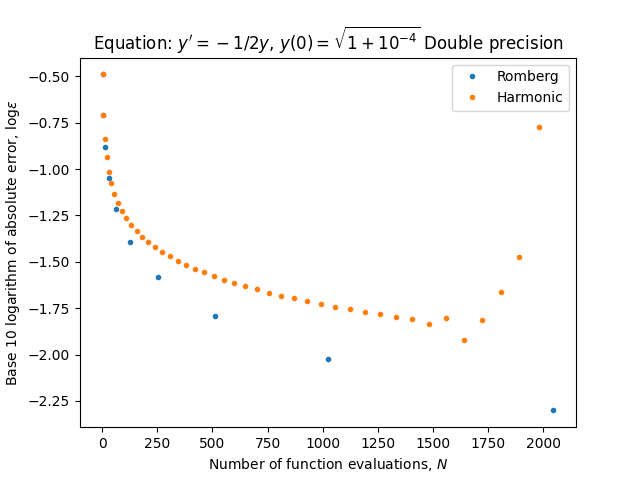
\includegraphics[scale=0.45]{emr_plots/quad_sing_4.png}
\end{minipage}
\begin{minipage}{0.45\textwidth}
\centering
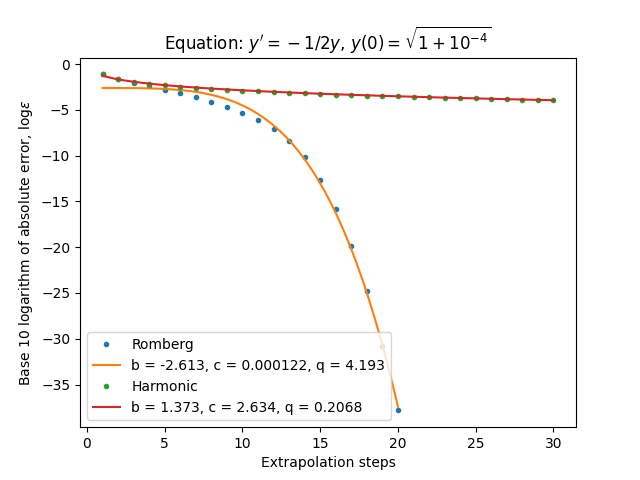
\includegraphics[scale=0.45]{emr_plots/quad_sing_4_hp_steps.png}
\end{minipage}
\end{figure}

\begin{figure}[H]
\centering
\begin{minipage}{0.45\textwidth}
\centering
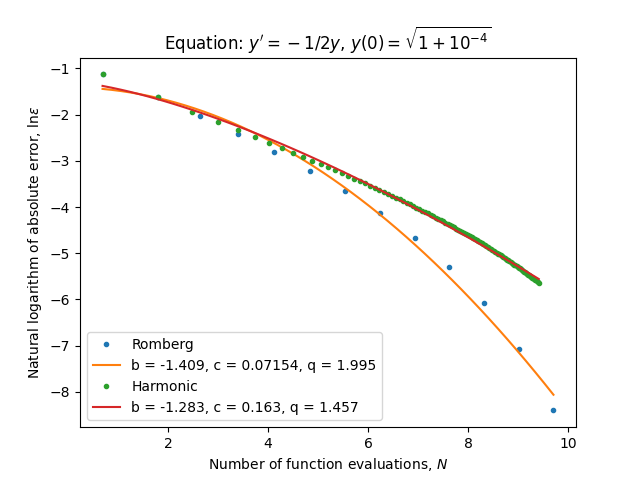
\includegraphics[scale=0.45]{emr_plots/quad_sing_4_hp_log_log_pow_fit_trend.png}
\end{minipage}
\begin{minipage}{0.45\textwidth}
\centering
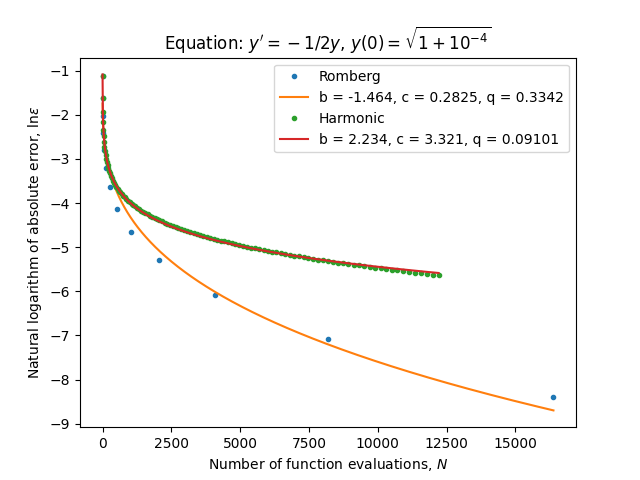
\includegraphics[scale=0.45]{emr_plots/quad_sing_4_hp_trend.png}
\end{minipage}
\end{figure}

\begin{table}[H]
    \centering
    \begin{tabular}{c|c||c|c|c}
Sequence & Plot & \(A\)-variance & \(c\)-variance & \(q\)-variance\\\hline
Romberg & lin-ln evals-error & \(1.0475\) & \(0.33656\) & \(0.080763\) \\
Harmonic & lin-ln evals-error & . & . & . \\
Romberg & lin-ln steps-error & \(0.19193\) & \(0.85108\) & \(0.055949\) \\
Harmonic & lin-ln steps-error & \(18.031\) & \(1.0619\) & \(0.12319\) \\
Romberg & ln-ln evals-error & \(0.19211\) & \(0.75886\) & \(0.052841\) \\
Harmonic & ln-ln evals-error & . & . & . \\
    \end{tabular}
    \label{tab:my_label}
\end{table}

The plot of \(q\) against \(a\) is as follows:

\begin{figure}[H]
\centering
\begin{minipage}{0.45\textwidth}
\centering
\includegraphics[scale=0.45]{emr_plots/log_p_vs_q_quad_sing.png}
\end{minipage}
\end{figure}

\subsection{Circular rotation}

Now we will consider the following system of equations:
\begin{equation}\label{48}
(y_1(t),y_2(t))' = (-y_2(t), y_1(t)), \quad y(0) = (1,0), \quad t\in [0,\pi /2]
\end{equation}
whose solution is 
\[
(y_1(t),y_2(t)) = (\cos t, \sin t)
\]
which is entire.

\begin{figure}[H]
\centering
\begin{minipage}{0.45\textwidth}
\centering
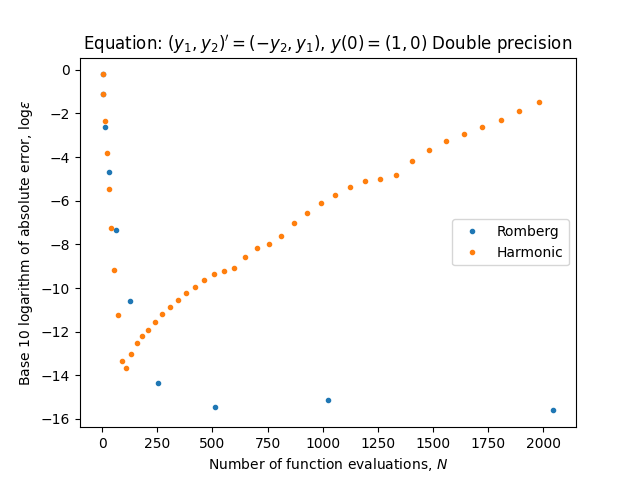
\includegraphics[scale=0.45]{emr_plots/rotation.png}
\end{minipage}
\begin{minipage}{0.45\textwidth}
\centering
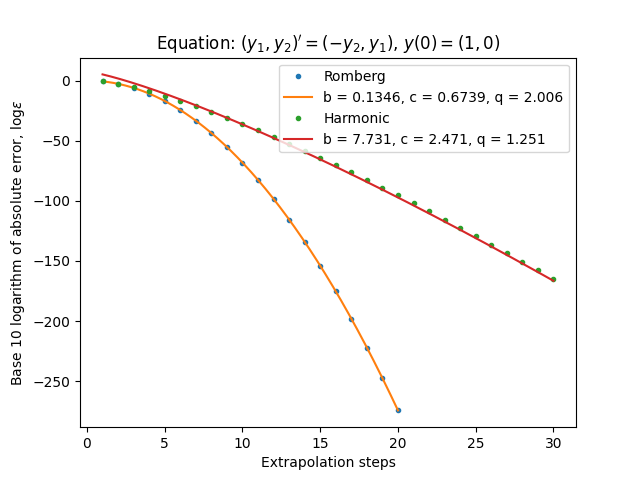
\includegraphics[scale=0.45]{emr_plots/rotation_hp_steps.png}
\end{minipage}
\end{figure}

\begin{figure}[H]
\centering
\begin{minipage}{0.45\textwidth}
\centering
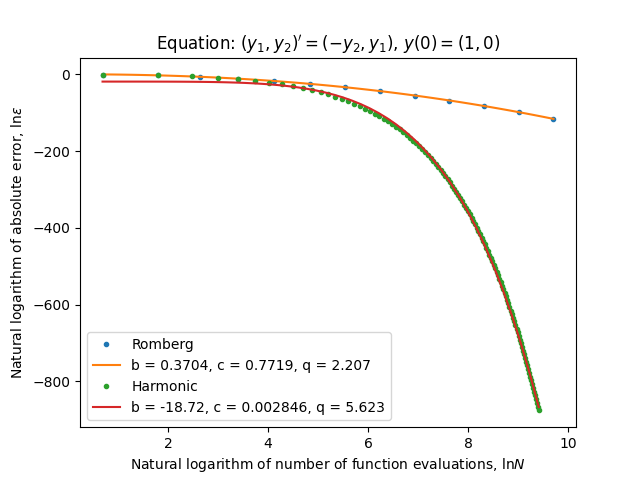
\includegraphics[scale=0.45]{emr_plots/rotation_hp_log_log_pow_fit_trend.png}
\end{minipage}
\begin{minipage}{0.45\textwidth}
\centering
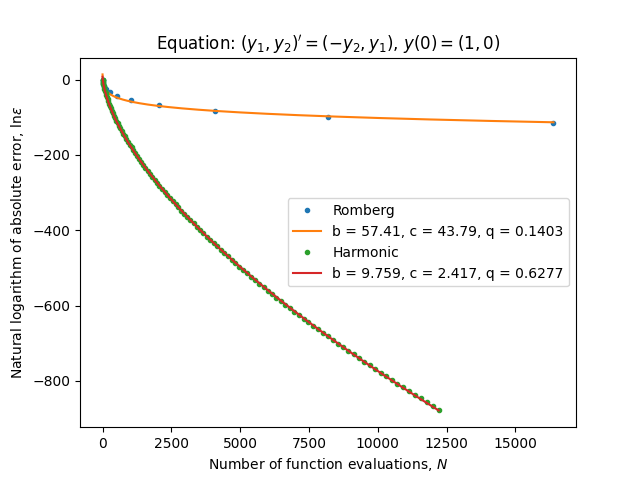
\includegraphics[scale=0.45]{emr_plots/rotation_hp_trend.png}
\end{minipage}
\end{figure}

\begin{table}[H]
    \centering
    \begin{tabular}{c|c||c|c|c}
Sequence & Plot & \(A\)-variance & \(c\)-variance & \(q\)-variance\\\hline
Romberg & lin-ln evals-error & \(3\) & \(0.10301\) & \(0.023866\) \\
Harmonic & lin-ln evals-error & \(12.976\) & \(0.0327\) & \(0.0016544\) \\
Romberg & lin-ln steps-error & \(0.00036387\) & \(6.2232e-06\) & \(2.3974e-07\) \\
Harmonic & lin-ln steps-error & \(12.521\) & \(0.027616\) & \(0.0013176\) \\
Romberg & ln-ln evals-error & \(0.34845\) & \(0.0052258\) & \(0.00022025\) \\
Harmonic & ln-ln evals-error & . & . & . \\
    \end{tabular}
    \label{tab:my_label}
\end{table}

The harmonic sequence works better then Romberg and we get down to machine level precision using either sequence when using standard floating point arithmetic.

\subsection{Mathematical pendulum}

Now we will consider the mathematical pendulum equation:
\begin{equation}
y''(t) + \sin y(t) = 0,\quad y(0) = 0,\, y'(0) = 1, \quad t\in [0,1].
\end{equation}

\begin{figure}[H]
\centering
\begin{minipage}{0.45\textwidth}
\centering
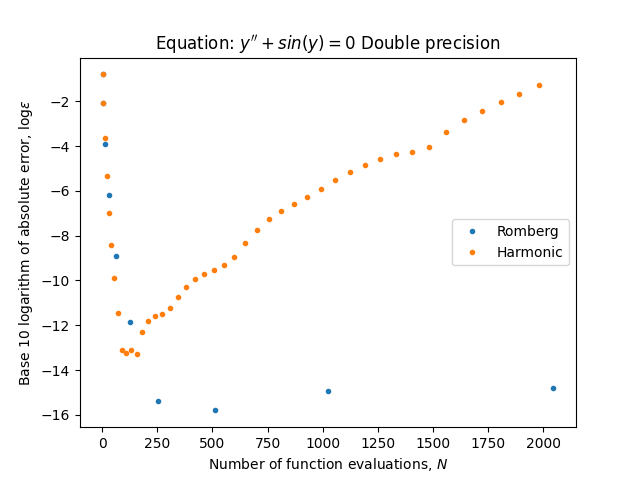
\includegraphics[scale=0.45]{emr_plots/oscillation.png}
\end{minipage}
\begin{minipage}{0.45\textwidth}
\centering
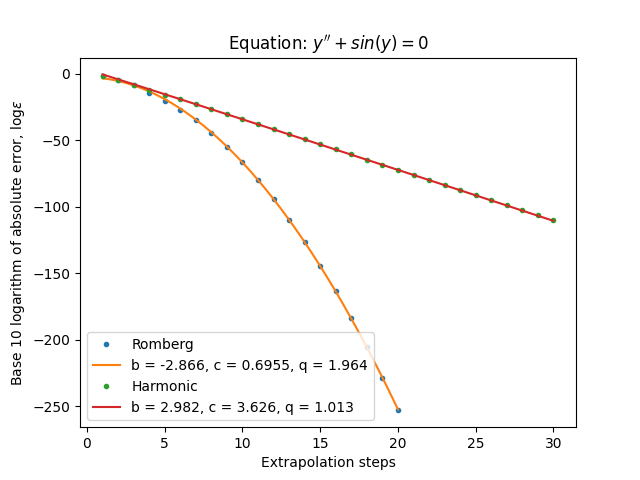
\includegraphics[scale=0.45]{emr_plots/oscillation_hp_steps.png}
\end{minipage}
\end{figure}

\begin{figure}[H]
\centering
\begin{minipage}{0.45\textwidth}
\centering
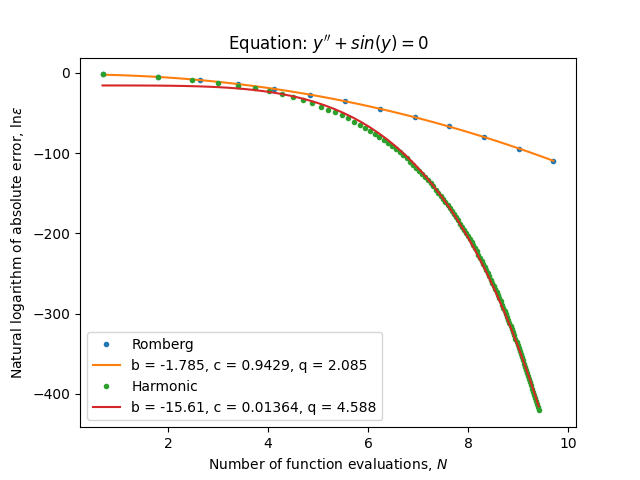
\includegraphics[scale=0.45]{emr_plots/oscillation_hp_log_log_pow_fit_trend.png}
\end{minipage}
\begin{minipage}{0.45\textwidth}
\centering
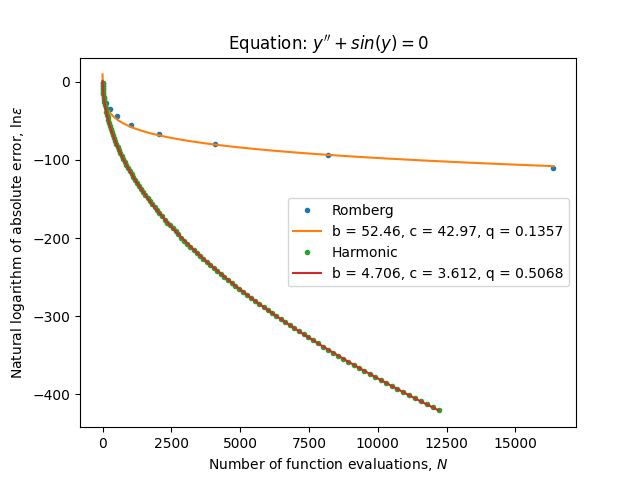
\includegraphics[scale=0.45]{emr_plots/oscillation_hp_trend.png}
\end{minipage}
\end{figure}

\begin{table}[H]
    \centering
    \begin{tabular}{c|c||c|c|c}
Sequence & Plot & \(A\)-variance & \(c\)-variance & \(q\)-variance\\\hline
Romberg & lin-ln evals-error & \(3\) & \(0.062258\) & \(0.011024\) \\
Harmonic & lin-ln evals-error & . & . & . \\
Romberg & lin-ln steps-error & \(1.6709\) & \(0.035263\) & \(0.001162\) \\
Harmonic & lin-ln steps-error & . & . & . \\
Romberg & ln-ln evals-error & \(0.74493\) & \(0.014052\) & \(0.00055219\) \\
Harmonic & ln-ln evals-error & . & . & . \\
    \end{tabular}
    \label{tab:my_label}
\end{table}

Here the model also fits very well, the harmonic sequence works better and we get down to machine level precision in standard floating point arithmetic, using either sequence.

\subsection{Federpendel}

Now we will consider the equation of motion for das Federpendel or the spring pendulum:
\[
\bfp' = -(|\bfq| - 1)\frac{\bfq}{|\bfq|} - {1\choose 0}, \quad \bfq' = \bfp
\]
where \(\bfp\) and \(\bfq\) are two dimensional vectors. We will consider it with the initial condition \(\bfq(0) = (1,0)\) and \(\bfp(0) = (0,1)\) and try to both estimate the solution at time \(t = 1\) and time \(t = 2\).

\begin{figure}[H]
\centering
\begin{minipage}{0.45\textwidth}
\centering
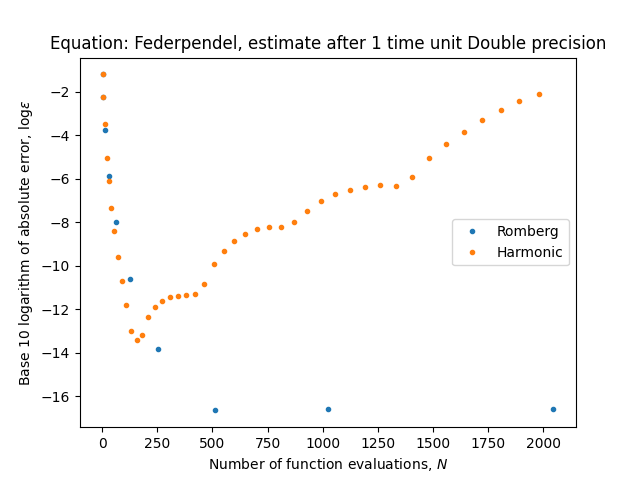
\includegraphics[scale=0.45]{emr_plots/federpendel.png}
\end{minipage}
\begin{minipage}{0.45\textwidth}
\centering
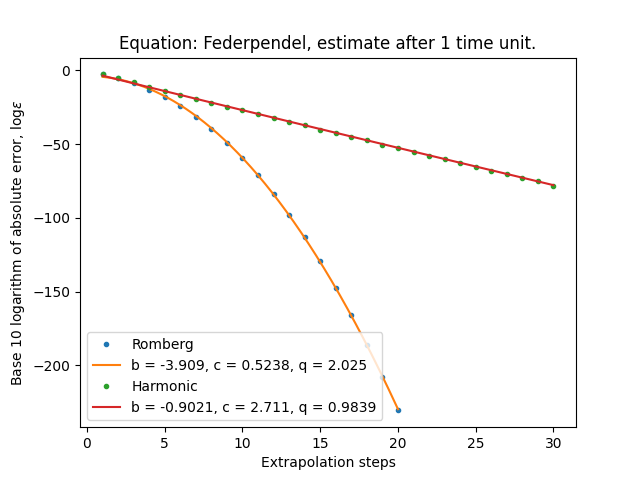
\includegraphics[scale=0.45]{emr_plots/federpendel_1_hp_steps.png}
\end{minipage}
\end{figure}

\begin{figure}[H]
\centering
\begin{minipage}{0.45\textwidth}
\centering
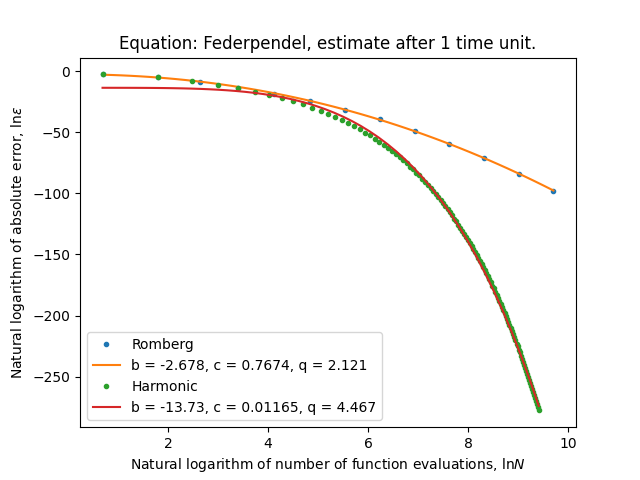
\includegraphics[scale=0.45]{emr_plots/federpendel_1_hp_log_log_pow_fit_trend.png}
\end{minipage}
\begin{minipage}{0.45\textwidth}
\centering
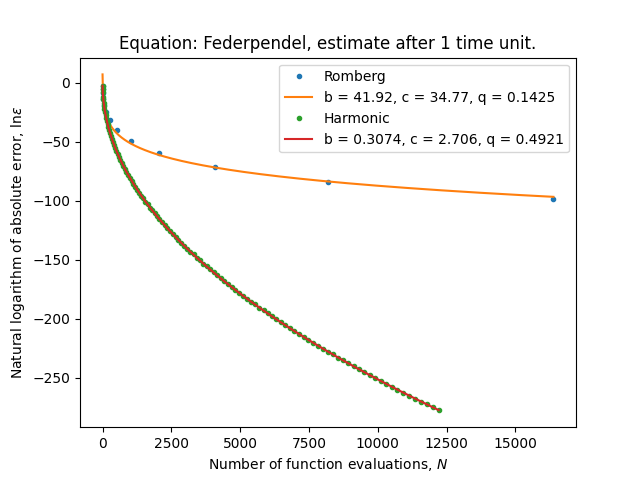
\includegraphics[scale=0.45]{emr_plots/federpendel_1_hp_trend.png}
\end{minipage}
\end{figure}

\begin{table}[H]
    \centering
    \begin{tabular}{c|c||c|c|c}
Sequence & Plot & \(A\)-variance & \(c\)-variance & \(q\)-variance\\\hline
Romberg & lin-ln evals-error & \(2.8972\) & \(0.073866\) & \(0.017293\) \\
Harmonic & lin-ln evals-error & . & . & . \\
Romberg & lin-ln steps-error & \(0.22658\) & \(0.0077523\) & \(0.00028806\) \\
Harmonic & lin-ln steps-error & . & . & . \\
Romberg & ln-ln evals-error & \(0.2334\) & \(0.0030672\) & \(0.00011101\) \\
Harmonic & ln-ln evals-error & . & . & . \\
    \end{tabular}
    \label{tab:my_label}
\end{table}


\begin{figure}[H]
\centering
\begin{minipage}{0.45\textwidth}
\centering
\includegraphics[scale=0.45]{emr_plots/federpendel_2.png}
\end{minipage}
\begin{minipage}{0.45\textwidth}
\centering
\includegraphics[scale=0.45]{emr_plots/federpendel_2_hp_steps.png}
\end{minipage}
\end{figure}

\begin{figure}[H]
\centering
\begin{minipage}{0.45\textwidth}
\centering
\includegraphics[scale=0.45]{emr_plots/federpendel_2_hp_log_log_pow_fit_trend.png}
\end{minipage}
\begin{minipage}{0.45\textwidth}
\centering
\includegraphics[scale=0.45]{emr_plots/federpendel_2_hp_trend.png}
\end{minipage}
\end{figure}

\begin{table}[H]
    \centering
    \begin{tabular}{c|c||c|c|c}
Sequence & Plot & \(A\)-variance & \(c\)-variance & \(q\)-variance\\\hline
Romberg & lin-ln evals-error & \(2.9999\) & \(0.17146\) & \(0.043627\) \\
Harmonic & lin-ln evals-error & . & . & . \\
Romberg & lin-ln steps-error & \(0.44685\) & \(0.040823\) & \(0.0016262\) \\
Harmonic & lin-ln steps-error & . & . & . \\
Romberg & ln-ln evals-error & \(0.66964\) & \(0.058913\) & \(0.0028387\) \\
Harmonic & ln-ln evals-error & . & . & . \\
    \end{tabular}
    \label{tab:my_label}
\end{table}

\subsection{Lorenz equations}

The Lorenz equations are the following system: 
\[
\frac{dx}{dt} = \sigma (y-x),\quad \frac{dy}{dt} = x(\rho - z) - y,\quad \frac{dz}{dt} = xy - \beta z
\]
where \(\sigma,\,\rho\) and \(\beta\) are constants. In our experiment, the constants are set to \(\sigma = 10\), \(\rho = 28\) and \(\beta = 8/3\). The initial condition we will consider is \((x(0),y(0),z(0)) = (1,1,1)\).\\

\begin{figure}[H]
\centering
\begin{minipage}{0.45\textwidth}
\centering
\includegraphics[scale=0.45]{emr_plots/lorenz.png}
\end{minipage}
\begin{minipage}{0.45\textwidth}
\centering
\includegraphics[scale=0.45]{emr_plots/lorenz_hp_steps.png}
\end{minipage}
\end{figure}

\begin{figure}[H]
\centering
\begin{minipage}{0.45\textwidth}
\centering
\includegraphics[scale=0.45]{emr_plots/lorenz_hp_log_log_pow_fit_trend.png}
\end{minipage}
\begin{minipage}{0.45\textwidth}
\centering
\includegraphics[scale=0.45]{emr_plots/lorenz_hp_trend.png}
\end{minipage}
\end{figure}

\begin{table}[H]
    \centering
    \begin{tabular}{c|c||c|c|c}
Sequence & Plot & \(A\)-variance & \(c\)-variance & \(q\)-variance\\\hline
Romberg & lin-ln evals-error & \(2.9999\) & \(0.12421\) & \(0.026917\) \\
Harmonic & lin-ln evals-error & . & . & . \\
Romberg & lin-ln steps-error & \(0.040351\) & \(0.00096717\) & \(3.4986e-05\) \\
Harmonic & lin-ln steps-error & . & . & . \\
Romberg & ln-ln evals-error & \(0.49281\) & \(0.011165\) & \(0.00044689\) \\
Harmonic & ln-ln evals-error & . & . & . \\
    \end{tabular}
    \label{tab:my_label}
\end{table}

\begin{figure}[H]
\centering
\begin{minipage}{0.45\textwidth}
\centering
\includegraphics[scale=0.45]{emr_plots/lorenz_02.png}
\end{minipage}
\begin{minipage}{0.45\textwidth}
\centering
\includegraphics[scale=0.45]{emr_plots/lorenz_02_hp_steps.png}
\end{minipage}
\end{figure}

\begin{figure}[H]
\centering
\begin{minipage}{0.45\textwidth}
\centering
\includegraphics[scale=0.45]{emr_plots/lorenz_02_hp_log_log_pow_fit_trend.png}
\end{minipage}
\begin{minipage}{0.45\textwidth}
\centering
\includegraphics[scale=0.45]{emr_plots/lorenz_02_hp_trend.png}
\end{minipage}
\end{figure}

\begin{table}[H]
    \centering
    \begin{tabular}{c|c||c|c|c}
Sequence & Plot & \(A\)-variance & \(c\)-variance & \(q\)-variance\\\hline
Romberg & lin-ln evals-error & \(2.9996\) & \(0.18327\) & \(0.034985\) \\
Harmonic & lin-ln evals-error & . & . & . \\
Romberg & lin-ln steps-error & \(0.33224\) & \(0.014775\) & \(0.00047548\) \\
Harmonic & lin-ln steps-error & . & . & . \\
Romberg & ln-ln evals-error & \(0.86945\) & \(0.038167\) & \(0.00137\) \\
Harmonic & ln-ln evals-error & . & . & . \\
    \end{tabular}
    \label{tab:my_label}
\end{table}

The model fits very well in both cases when we consider the number of evaluations against error. The harmonic sequence works better. The fitting is not as nice when considering the number of extrapolation seps against the error. In standard floating point arithmetic, we obtain higher accurracy using the Romberg sequence, though we get high accurracy in both cases.\\

The values of the optimal parameters in the fitting of the number evaluations against the error, are:

\begin{table}[H]
    \centering
    \begin{tabular}{c|c||c|c|c}
           IVP & Sequence & \(b\) & \(c\) & \(q\) \\\hline\hline
$y'=y$, $y(0) = 0$ & Romberg & \(27.187\) & \(22.015\) & \(0.20227\) \\
$y'=y$, $y(0) = 0$ & Harmonic & \(8.8124\) & \(3.0433\) & \(0.61436\) \\
$y' = y(1-y)$ & Romberg & \(17.604\) & \(19.237\) & \(0.20418\) \\
$y' = y(1-y)$ & Harmonic & \(1.7927\) & \(4.0933\) & \(0.51064\) \\
$y' = 1 + y^2$, $y(0) = 0$ & Romberg & \(11.465\) & \(8.8186\) & \(0.24549\) \\
$y' = 1 + y^2$, $y(0) = 0$ & Harmonic & \(3.3496\) & \(1.8647\) & \(0.51993\) \\
$(y_1,y_2)' = (-y_2,y_1)$, $y(0) = (1,0)$ & Romberg & \(22.626\) & \(16.846\) & \(0.2184\) \\
$(y_1,y_2)' = (-y_2,y_1)$, $y(0) = (1,0)$ & Harmonic & \(9.7592\) & \(2.4171\) & \(0.62765\) \\
$y' = y^2$, $y(0) = 1/2$ & Romberg & \(14.78\) & \(12.517\) & \(0.22455\) \\
$y' = y^2$, $y(0) = 1/2$ & Harmonic & \(3.5994\) & \(2.5894\) & \(0.51472\) \\
$y'=y^2$, $y(0) = 1/(1+10^{-2})$ & Romberg & \(5.3983\) & \(0.1961\) & \(0.4989\) \\
$y'=y^2$, $y(0) = 1/(1+10^{-2})$ & Harmonic & \(4.7796\) & \(0.032416\) & \(0.6592\) \\
$y'=y^2$, $y(0) = 1/(1+10^{-4})$ & Romberg & \(9.212\) & \(0.00012308\) & \(0.94461\) \\
$y'=y^2$, $y(0) = 1/(1+10^{-4})$ & Harmonic & \(9.2104\) & \(0.00016925\) & \(0.74975\) \\
$y' = -1/2y$, $y(0) = \sqrt{2}$ & Romberg & \(17.142\) & \(17.376\) & \(0.2007\) \\
$y' = -1/2y$, $y(0) = \sqrt{2}$ & Harmonic & \(-0.45512\) & \(3.1436\) & \(0.49744\) \\
$y' = -1/2y$, $y(0) = \sqrt{1+10^{-2}}$ & Romberg & \(0.063222\) & \(1.0479\) & \(0.35645\) \\
$y' = -1/2y$, $y(0) = \sqrt{1+10^{-2}}$ & Harmonic & \(-1.7425\) & \(0.33371\) & \(0.45544\) \\
$y' = -1/2y$, $y(0) = \sqrt{1+10^{-4}}$ & Romberg & \(0.13652\) & \(1.2653\) & \(0.19436\) \\
$y' = -1/2y$, $y(0) = \sqrt{1+10^{-4}}$ & Harmonic & \(2.2343\) & \(3.3206\) & \(0.091009\) \\
$y'' + \sin(y) = 0$ & Romberg & \(22.275\) & \(19.017\) & \(0.20078\) \\
$y'' + \sin(y) = 0$ & Harmonic & \(4.7064\) & \(3.6116\) & \(0.50678\) \\
Federpendel, estimate after 1 time unit. & Romberg & \(17.532\) & \(15.778\) & \(0.20624\) \\
Federpendel, estimate after 1 time unit. & Harmonic & \(0.30737\) & \(2.706\) & \(0.49211\) \\
Federpendel, estimate after 2 time units. & Romberg & \(14.66\) & \(11.217\) & \(0.22272\) \\
Federpendel, estimate after 2 time units. & Harmonic & \(0.79006\) & \(1.789\) & \(0.48379\) \\
Lorenz, estimate after 0.1 time steps. & Romberg & \(18.654\) & \(12.939\) & \(0.2354\) \\
Lorenz, estimate after 0.1 time steps. & Harmonic & \(12.615\) & \(4.0068\) & \(0.5111\) \\
Lorenz, estimate after 0.2 time steps. & Romberg & \(14.264\) & \(7.2173\) & \(0.27063\) \\
Lorenz, estimate after 0.2 time steps. & Harmonic & \(13.212\) & \(2.7376\) & \(0.50732\) \\
    \end{tabular}
    \caption{Optimal parameters by test case}
    \label{tab:my_label}
\end{table}

We note that in those cases where the singularities of the solutions are not very close to our time interval, then \(q\) is close to \(0.5\) for the harmonic sequence and close to \(0.2\) for the Romberg sequence.\\

The values of the optimal parameters in the fitting of the number of extrapolation steps against the error, are:

\begin{table}[H]
    \centering
    \begin{tabular}{c|c||c|c|c}
           IVP & Sequence & \(b\) & \(c\) & \(q\) \\\hline\hline
$y'=y$, $y(0) = 0$ & Romberg & \(-1.0083\) & \(0.9557\) & \(1.904\) \\
$y'=y$, $y(0) = 0$ & Harmonic & \(6.425\) & \(3.1061\) & \(1.225\) \\
$y' = y(1-y)$ & Romberg & \(-7.1901\) & \(0.82672\) & \(1.916\) \\
$y' = y(1-y)$ & Harmonic & \(-0.19572\) & \(4.1127\) & \(1.0204\) \\
$y' = 1 + y^2$, $y(0) = 0$ & Romberg & \(-1.2103\) & \(0.30542\) & \(2.1771\) \\
$y' = 1 + y^2$, $y(0) = 0$ & Harmonic & \(2.405\) & \(1.8763\) & \(1.0387\) \\
$(y_1,y_2)' = (-y_2,y_1)$, $y(0) = (1,0)$ & Romberg & \(0.15924\) & \(0.67746\) & \(2.004\) \\
$(y_1,y_2)' = (-y_2,y_1)$, $y(0) = (1,0)$ & Harmonic & \(7.7307\) & \(2.4712\) & \(1.2513\) \\
$y' = y^2$, $y(0) = 1/2$ & Romberg & \(-2.193\) & \(0.48799\) & \(2.0424\) \\
$y' = y^2$, $y(0) = 1/2$ & Harmonic & \(2.3181\) & \(2.6033\) & \(1.0284\) \\
$y'=y^2$, $y(0) = 1/(1+10^{-2})$ & Romberg & \(4.6269\) & \(0.00074557\) & \(4.042\) \\
$y'=y^2$, $y(0) = 1/(1+10^{-2})$ & Harmonic & \(4.7474\) & \(0.033263\) & \(1.3137\) \\
$y'=y^2$, $y(0) = 1/(1+10^{-4})$ & Romberg & \(-2507.7\) & \(-2517.1\) & \(-0.00010114\) \\
$y'=y^2$, $y(0) = 1/(1+10^{-4})$ & Harmonic & \(9.2101\) & \(0.00017545\) & \(1.4929\) \\
$y' = -1/2y$, $y(0) = \sqrt{2}$ & Romberg & \(-5.0269\) & \(0.76221\) & \(1.8929\) \\
$y' = -1/2y$, $y(0) = \sqrt{2}$ & Harmonic & \(-1.8945\) & \(3.1518\) & \(0.99437\) \\
$y' = -1/2y$, $y(0) = \sqrt{1+10^{-2}}$ & Romberg & \(-2.1638\) & \(0.015532\) & \(2.9565\) \\
$y' = -1/2y$, $y(0) = \sqrt{1+10^{-2}}$ & Harmonic & \(-1.8689\) & \(0.33241\) & \(0.91148\) \\
$y' = -1/2y$, $y(0) = \sqrt{1+10^{-4}}$ & Romberg & \(-1.4291\) & \(0.062542\) & \(1.8173\) \\
$y' = -1/2y$, $y(0) = \sqrt{1+10^{-4}}$ & Harmonic & \(1.3726\) & \(2.6336\) & \(0.20682\) \\
$y'' + \sin(y) = 0$ & Romberg & \(-1.9686\) & \(0.83745\) & \(1.8917\) \\
$y'' + \sin(y) = 0$ & Harmonic & \(2.9822\) & \(3.6265\) & \(1.0128\) \\
Federpendel, estimate after 1 time unit. & Romberg & \(-2.8486\) & \(0.67856\) & \(1.9249\) \\
Federpendel, estimate after 1 time unit. & Harmonic & \(-0.90208\) & \(2.7108\) & \(0.98385\) \\
Federpendel, estimate after 2 time units. & Romberg & \(-0.45874\) & \(0.44537\) & \(2.0272\) \\
Federpendel, estimate after 2 time units. & Harmonic & \(0.020877\) & \(1.79\) & \(0.96743\) \\
Lorenz, estimate after 0.1 time steps. & Romberg & \(0.59151\) & \(0.47509\) & \(2.112\) \\
Lorenz, estimate after 0.1 time steps. & Harmonic & \(10.659\) & \(4.0254\) & \(1.0213\) \\
Lorenz, estimate after 0.2 time steps. & Romberg & \(3.1116\) & \(0.21429\) & \(2.3417\) \\
Lorenz, estimate after 0.2 time steps. & Harmonic & \(11.891\) & \(2.7477\) & \(1.014\) \\
    \end{tabular}
    \caption{Optimal parameters by test case}
    \label{tab:my_label}
\end{table}